\documentclass[]{scrartcl}
\usepackage{graphicx}
%\pagestyle{headings}

\begin{document}

\title{Sensory Analysis}
\subtitle{brewing lecture at TU-Berlin}
\author{Christopher Weyand}
\maketitle
\begin{abstract}
Brewing is a widespread field including the scientific disciple of sensory analysis
that, for the purpose of evaluating consumer products, applies principles of experimental
design and statistical analysis to the use of human senses.
\end{abstract}
\newpage

\tableofcontents
\newpage

\listoffigures
\newpage


\section{Main Goals}
\begin{enumerate}
  \item Comparison
  \item Description
  \item Preference
\end{enumerate}


\section{Definition of Sensory Analysis}
A sensory evaluation is performed to detect, identify and evaluate
characteristics of products utilizing all of the sensory pathways.
(olfactory, visual, gustatory, auditory, tactile)


\section{Sensory Perception}
\subsection{Gustatory Analysis}
The main flavors are:
\begin{itemize}
  \item salty
  \item sweet
  \item bitter
  \item sour
\end{itemize}

\subsection{Olfactory Analysis}
The olfactory sense offers a direct connection to our brainstem through the trigeminal nerve.
Thus the signal processing of olfactory input to our brain is not located in the cerebrum.
Evolutionary smelling is the first developed sense. Like bakteria communicates with semiochemicals
- called quorum sensing - animals utilize special scents to find a mate or lokate their enemy. Also the olfactory
vomeronasal organ found in many animals lies close to the nasal bones.

The markedness of the olfactory sense deeply depends on cultural and regional influences.
An asian might reject a Limburger cheese in disgust while a human raised in the western european
counties enjoys it's intense fragrance.

durian: frucht aus südostasien wird königin der früchte genannt,
stinkende reudige frucht, in asien beliebt, im flugzeug verboten, richt sehr intensiv

\subsection{Tactile Analysis}
\begin{itemize}
  \item tingling
  \item viscosity
  \item temperature
\end{itemize}


\section{Testing Methods}
Below follows a section about the methods of sensory testing in scientific environments.
They are listed in alphabetical order.
\subsection{authenticity test}
Does the product meet customer expectations.

\subsection{aversion test}
This test is a prederence test that permits just like or dislike as an answer.

\subsection{blind test}
The test subjects are left in the dark about the type or brand of the sample.

\subsection{branded test}
The branded test is the counterpart to the blind test.

\subsection{descriptive testing}
QDA: quantitative descriptive analysis

\subsection{difference tests}
Difference tests include the difference ranking test.

\subsection{duo-trio test}
It is to determine with wich of two original samples a third sample matches.

\subsection{hedonic test}
Hedonic or affective tests are simple processes to determine ones preferences offering
just a few options to chose from.

\subsection{monadic test}
The monadic test is done using just one sample and no comparison.

\subsection{threshold test}
//todo

\subsection{time intensity test}
Refers to the behavior of sensory impressions like bitter -or tardness over time
as seen in figure \ref{fig:time-intensity}.
\begin{figure}[h]
	\centering
	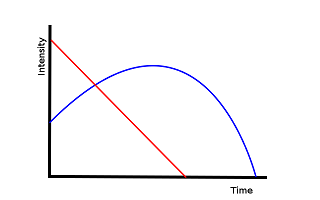
\includegraphics{time-intensity.png}
	\caption{intensity of sensory impression over time}
	\label{fig:time-intensity}
\end{figure}

\subsection{triangle test}
//todo


\section{Identification of the basic Flavor Types}
sweet \newline
4.5 g/l sugar \newline
bitter \newline
0,7 g/l caffeine \newline
sour \newline
0.4 g/l citric acid \newline
salty \newline
0.9 g/l sodium chloride \newline


\newpage
\section{Miscellaneous}
Before Sensorik you shall not:
\begin{itemize}
  \item smoke
  \item eat chocolate
  \item use perfume
  \item forget to shower
\end{itemize}
Also women are more sensitive to olfactory impulses. Furthermore they gustatory perceive
more intense in special ways including the bitterness. This leads to aversion of bitter beer
by most women.

knäckebrot zwischen verkostungen sehr gut zum neutralisieren, wasser
baguette oder weizenmehlbrötchen ohne geschmacksstoffe (schlecht zb. sesambrötchen)
falls kein brot min. 20-30 sec zw. proben warten, speichel sammeln
überlagerungseffekte vermeiden
zucker hat geschmacksverstärkende wirkung, was zu fehlinterpretationen führen kann
konzentration ist enorm wichtig, sensibilität steigt mit konzentration auf die eigenen sinne
nicht auf andere achten
nicht rauchen, weil nicotin nerven betäubt und die geschmacksstoffe im rauch den
eindruck einer sensorischen analyse beeinflussen



bier braucht schaumkrone -> egal ob aussehen, geschmack, temperatur ... gut ist (ausser man ist am verdursten)
professor hat köstrizer schwazbier entwickelt in den 90ern
	schwarzbier war marktlücke
	gab nur guinnes und könig ludwig dunkel
		meinungen zu guinnes waren sehr extrem, love or hate
	studentenpanel zur auswertung genutzt

sensorik dient dazu die qualität von lebensmitteln zu ermitteln, falls analytische methoden nicht anwendbar sind
der allgemeine geschmackseindruck eines biers ist von so vielen faktoren abhängig, dass man es schwer analytisch eingrenzen kann
synergistische und überlagerungseffekte sind messtechnisch nicht gut abschätzbar
oxidationsprodukte von minorkomponenten können sensorisches bild beeinflussen

voraussetzungen der sensorischen analyse
	wahrnehmung eines geschmackseindrucks
	reproduzierbarkeit
	um das zu erreichen benötigt es definierte bedingungen
	methodik angemessen für zielsetzung
	trainiertes panel -> hauptfokus der sensorik ist verbesserung der sensibilisierung (verkostung durchgeführt von fachleuten)

Link between consumer and product:
consumer panel
	leihen
	kein besonderen voraussetzungen
descriptive panel
	trainierte geschulte tester
	in der lage geschmackseindruck professionell wiederzugeben
SA eingesetzt für marketing und market research oder product research, development









\end{document}
